\documentclass[aspectratio=169]{beamer}

\usetheme{Madrid}
% Remove the default parentheses around the institute in the footline
\setbeamertemplate{footline}{%
  \leavevmode%
  \hbox{%
    \begin{beamercolorbox}[wd=.33\paperwidth,ht=2.5ex,dp=1.125ex,leftskip=.3cm]{author in head/foot}%
      \usebeamerfont{author in head/foot}\insertshortauthor
    \end{beamercolorbox}%
    \begin{beamercolorbox}[wd=.34\paperwidth,ht=2.5ex,dp=1.125ex,center]{title in head/foot}%
      \usebeamerfont{title in head/foot}\insertshorttitle
    \end{beamercolorbox}%
    \begin{beamercolorbox}[wd=.33\paperwidth,ht=2.5ex,dp=1.125ex,rightskip=.3cm plus1fil]{date in head/foot}%
      \usebeamerfont{date in head/foot}\insertshortinstitute\hfill\insertframenumber/\inserttotalframenumber
    \end{beamercolorbox}%
  }%
}

\usepackage{amsmath,amssymb}
\usepackage{graphicx}

\usepackage{booktabs}
\usepackage{array}
\usepackage{siunitx}
\sisetup{detect-all}

\usepackage{tikz}
\usetikzlibrary{arrows.meta,positioning,fit,calc}

\usepackage[most]{tcolorbox}
\tcbset{colback=gray!6,colframe=black!35,boxrule=0.6pt,arc=2pt}

% beamer already loads hyperref; configure it here to avoid option clashes
\hypersetup{hidelinks}

\title[IFRS 17 Actuarial Audit]{Introduction to Actuarial Audit under IFRS~17}
\author{Leonardo Valentino Kosasih}
\institute{Institut Teknologi Bandung}
\date{\today}

% Section divider at the start of each agenda section
\AtBeginSection[]{
  \begin{frame}[plain,noframenumbering]
    \vfill
    \begin{center}
      {\LARGE \insertsectionhead}

      \vspace{0.4em}
      {\large IFRS~17 actuarial audit}
    \end{center}
    \vfill
  \end{frame}
}

\begin{document}

\begin{frame}
  \titlepage
\end{frame}

\begin{frame}{Agenda}
  \begin{enumerate}
    \item Actuarial Science and Accounting
    \item What is an Insurance Contract
    \item LfRC (Liability for Remaining Coverage)
    \item LfIC (Liability for Incurred Claims)
    \item Financial Disclosure 
  \end{enumerate}
\end{frame}
\begin{frame}{Out of Scope}
\begin{enumerate}
\item Reinsurance Contract Held
\item Shariah Insurance
\end{enumerate}
\end{frame}
\begin{frame}{My Personal Goal from Today's Session}
\begin{enumerate}
  \item Sharing 30\% accounting knowledge 70\% actuarial application
  \item Showing you some memes along the presentation so keep your eyes open :D
  \item Audit is about how you think, not just what you do.
  \item \text{ }
    \begin{center}
      
\includegraphics[width=0.65\linewidth,height=0.38\textheight,keepaspectratio]{cinema.jpeg}
    \end{center}
\end{enumerate}
\end{frame}
\section{Actuarial Science and Accounting}

\begin{frame}{Actuaries and Accountants}
  \vspace{-0.3em}
  \begin{columns}[T,onlytextwidth]
    \column{0.5\textwidth}
      \centering
      
\includegraphics[width=\linewidth,height=0.68\textheight,keepaspectratio]{meme-accountant-actuary-1.jpg}

    \column{0.5\textwidth}
      \centering
      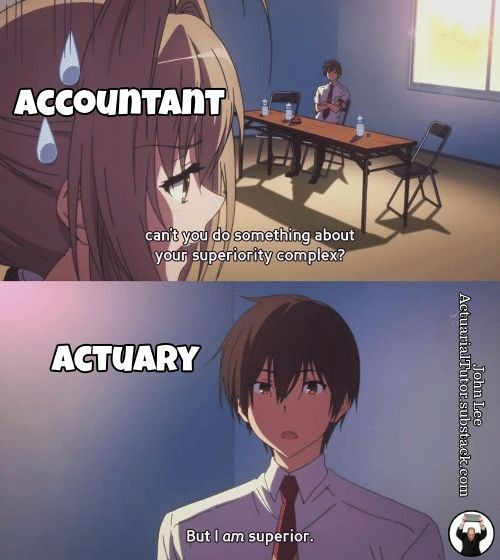
\includegraphics[width=\linewidth,height=0.68\textheight,keepaspectratio]{meme-accountant-actuary-2.jpg}
  \end{columns}

  \vspace{0.3em}
  \footnotesize
  Why do these memes exist? Is it true? (Credit to:\href{https://actuarialtutor.uk/memes/}{John Lee})
\end{frame}

\begin{frame}{Accounting Standars for Insurance} 
In (re)insurance one of the International Financial Reporting Standards (IFRS) we use is IFRS 17 : Insurance Contract. In every IFRS, it has 3 major sections:
\begin{enumerate}
  \item Scope: which items are covered by the IFRS (accounting),
  \item Recognition and Measurement: how to record the initial balance (actuarial science),
  \item Disclosure: how to present the result in financial disclosures (accounting).
\end{enumerate}
Doing the actuarial audit, means that we need to check the documentation, assumptions used and whether it align with the standards.
\end{frame}

\begin{frame}{Example of IFRS17 Financial Statement - Balance Sheet}
Below is the Prudential Life \href{https://www.prudentialplc.com/en/newsroom/company-news/2025/prudential-plc-2024-full-year-results/}{IFRS17 disclosure} access on 6 February 2026.

  \begin{columns}[T,onlytextwidth]
    \column{0.5\textwidth}
      \centering
      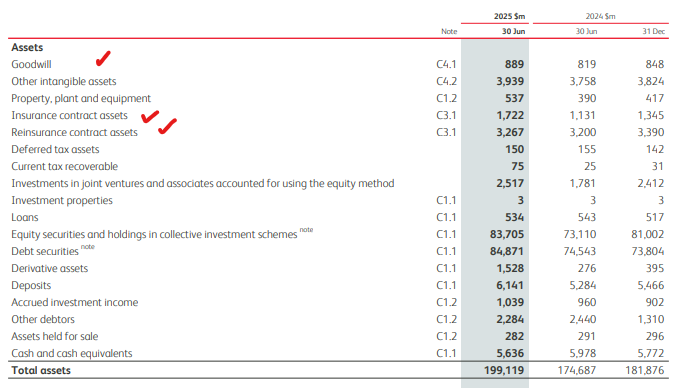
\includegraphics[width=0.98\linewidth,height=0.78\textheight,keepaspectratio]{FS Prudential - Asset.png}

    \column{0.5\textwidth}
      \centering
      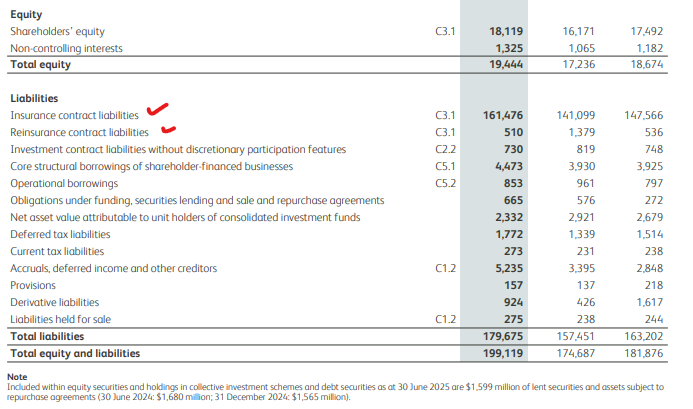
\includegraphics[width=0.98\linewidth,height=0.78\textheight,keepaspectratio]{FS Prudential - Liabilities and Equity.png}
  \end{columns}
Observe that the Insurance Contract Liabilities (ICL) is around 80\% of the total equity and liabilities, which make it more important to verify whether the amount is correct.
\end{frame}

\begin{frame}{Example of IFRS17 Financial Statement - Profit and Loss}
  \begin{center}
  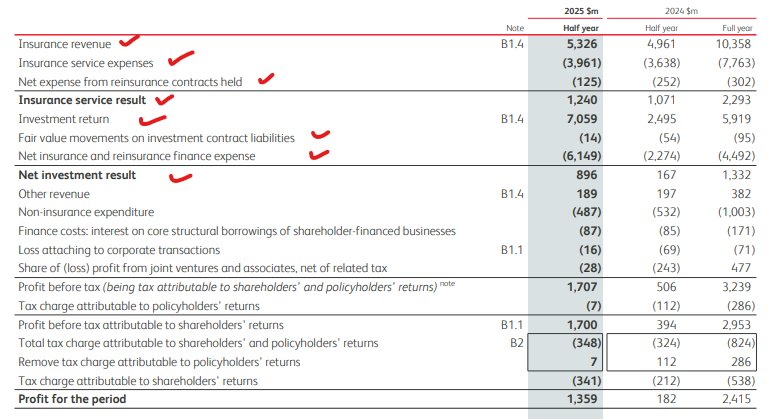
\includegraphics[width=0.90\linewidth,height=0.7\textheight,keepaspectratio]{PL Prudential.png}
  \end{center} 
Top 4 of the largest line items are investment return, net insurance and reinsurance finance epxense insurance revenue and insurance service expenses
\end{frame}


\section{What is an Insurance Contract}

\begin{frame}{Introduction to Insurance Contract}
  \textbf{Insurance contract} is a contract under which one party (the issuer) accepts \textbf{significant insurance risk} from another party (the policyholder) by agreeing to \textbf{compensate} the policyholder if a specified \textbf{uncertain future event} (the insured event) adversely affects the policyholder.

  \vspace{0.2em}
  \footnotesize
  \textit{Source: IFRS~17, Appendix A (Definitions).}

  \vspace{0.4em}
  \normalsize
  Typical lifecycle of an insurance as a policyholder:

  \vspace{0.2em}
  \begin{center}
  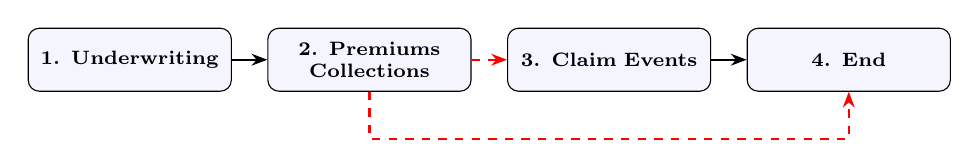
\begin{tikzpicture}[
    node distance=0mm and 4.5mm,
    box/.style={draw, rounded corners, align=center, fill=blue!4, inner sep=2.2pt, font=\scriptsize, text width=0.20\linewidth, minimum height=8mm},
    arr/.style={-{Stealth[length=2.0mm]}, thick}
  ]
    \node[box] (uw) {\textbf{1. Underwriting}};
    \node[box, right=of uw] (prem) {\textbf{2. Premiums Collections}};
    \node[box, right=of prem] (claims) {\textbf{3. Claim Events}};
    \node[box, right=of claims] (end) {\textbf{4. End}};

    \draw[arr] (uw) -- (prem);
    \draw[dashed, thick, red, -{Stealth[length=2.0mm]}] (prem.south) -- ++(0,-6mm) -| (end.south);
    \draw[dashed, thick, red, -{Stealth[length=2.0mm]}] (prem) -- (claims);
    \draw[arr] (claims) -- (end);
  \end{tikzpicture}
  \end{center}
But how to determine the \textbf{significant insurance risk}?
\end{frame}
\begin{frame}[allowframebreaks]{What is an insurance contract (conceptually)?}
Insurance risk is significant if and only if, an insured event could cause the issuer to pay \textbf{additional amounts} that are significant in any single scenario, excluding scenarios that have no commercial substance (i.e., no discernible effect on the economics of the transaction)... 
\footnotesize
\textit{Source: IFRS~17, Appendix B18}
\normalsize

The additional amounts above are determined on a present-value basis.

\footnotesize
\textit{Source: IFRS~17, Appendix B20}
\normalsize

\framebreak
\textbf{The additional ammounts} refer to the present value of amounts that exceed those that would be payable if no insured event had occurred (excluding scenarios that lack commercial substance). Those additional amounts include claims handling and assessment costs, but exclude:
\begin{itemize}
  \item the loss of the ability to charge the policyholder for future service, 
  \item a waiver, on death, of charges that would be made on cancellation or surrender, %for example death due to war, suicide, the terms that make the contract invalid
  \item a payment conditional on an event that does not cause a significant loss to the holder of the contract, 
  \item possible reinsurance recoveries.
\end{itemize}

\footnotesize
\textit{Source: IFRS~17, Appendix B21}
\normalsize

Or as an actuary, this means to:
\begin{equation}
\frac{\sum_{i} E\[\text{PVCF}_{i,\text{ claim event}\]}}{\sum_{i} E\[\text{PVCF}_{i,\text{ no claim event}\]}}
\end{equation}
\end{frame}

\begin{frame}{Quick Break}
From this section, now you know how to answer this question from a very famous \textit{"star"}
\begin{center}

\includegraphics[width=0.90\linewidth,height=0.7\textheight,keepaspectratio]{Patrick Mayonnaise.png}
\end{center}
\end{frame}

\section{LfRC (Liability for Remaining Coverage)}

\begin{frame}{Where's My Money}
  \begin{center}
  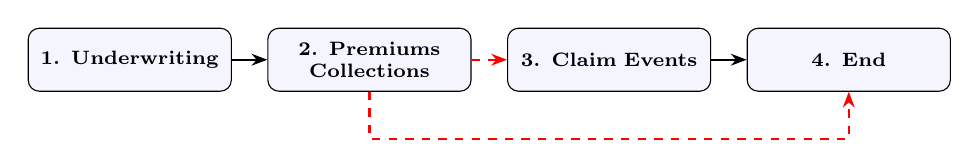
\begin{tikzpicture}[
    node distance=0mm and 4.5mm,
    box/.style={draw, rounded corners, align=center, fill=blue!4, inner sep=2.2pt, font=\scriptsize, text width=0.20\linewidth, minimum height=8mm},
    arr/.style={-{Stealth[length=2.0mm]}, thick}
  ]
    \node[box] (uw) {\textbf{1. Underwriting}};
    \node[box, right=of uw] (prem) {\textbf{2. Premiums Collections}};
    \node[box, right=of prem] (claims) {\textbf{3. Claim Events}};
    \node[box, right=of claims] (end) {\textbf{4. End}};

    \draw[arr] (uw) -- (prem);
    \draw[dashed, thick, red, -{Stealth[length=2.0mm]}] (prem.south) -- ++(0,-6mm) -| (end.south);
    \draw[dashed, thick, red, -{Stealth[length=2.0mm]}] (prem) -- (claims);
    \draw[arr] (claims) -- (end);
  \end{tikzpicture}
  \end{center}
We are going to take a closer look on the lifecyle of an insurance from previous slide and ask ourselves, "what happened to the money after policyholders pay the premium? Does the insurer just keep the money in a bank? Pay claims to other policyholder? or just hope that no claim will submitted ?\\
When the insurance are issued, the insurance directly become a liability of the insurrer meaning that the insurance company is liable to pay the policy holder if a claim event happened. But it doesn't mean that every insurance will be a libility to the insurance company. There will be some cases where the insurance can be an assets (as we see in the previous balance sheet example).
\end{frame}

\begin{frame}{What's inside the Insurance Contract Liability (ICL)?}
  \vspace{0.2em}
  \begin{center}
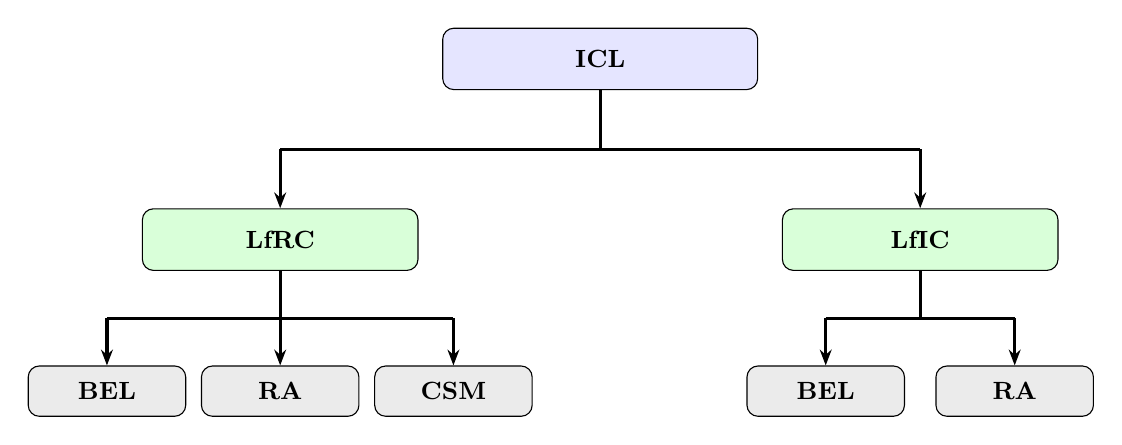
\begin{tikzpicture}[
  font=\small,
  main/.style={draw, rounded corners, fill=blue!10, inner sep=8pt, align=center, minimum width=40mm},
  mid/.style={draw, rounded corners, fill=green!15, inner sep=8pt, align=center, minimum width=35mm},
  leaf/.style={draw, rounded corners, fill=black!8, inner sep=6pt, align=center, minimum width=20mm},
  bar/.style={line width=1.2pt},
  arr/.style={-{Stealth[length=2mm]}, line width=1.2pt}
]
  % Top level
  \node[main] (icl) {\textbf{ICL}};
  
  % Two main components - positioned manually for exact control
  \node[mid, below left=15mm and 3mm of icl] (lfrc) {\textbf{LfRC}};
  \node[mid, below right=15mm and 3mm of icl] (lfic) {\textbf{LfIC}};
  
  % Split from ICL
  \coordinate (split1) at ($(icl.south)+(0,-7.5mm)$);
  \draw[bar] (icl.south) -- (split1);
  \draw[bar] (split1 -| lfrc) -- (split1 -| lfic);
  \draw[arr] (split1 -| lfrc) -- (lfrc.north);
  \draw[arr] (split1 -| lfic) -- (lfic.north);
  
  % LfRC breakdown: BEL, RA, CSM (3 equal boxes)
  \node[leaf, below=12mm of lfrc, xshift=-22mm] (lfrc-bel) {\textbf{BEL}};
  \node[leaf, below=12mm of lfrc] (lfrc-ra) {\textbf{RA}};
  \node[leaf, below=12mm of lfrc, xshift=22mm] (lfrc-csm) {\textbf{CSM}};
  
  \coordinate (split2) at ($(lfrc.south)+(0,-6mm)$);
  \draw[bar] (lfrc.south) -- (split2);
  \draw[bar] (split2 -| lfrc-bel) -- (split2 -| lfrc-csm);
  \draw[arr] (split2 -| lfrc-bel) -- (lfrc-bel.north);
  \draw[arr] (split2 -| lfrc-ra) -- (lfrc-ra.north);
  \draw[arr] (split2 -| lfrc-csm) -- (lfrc-csm.north);
  
  % LfIC breakdown: only BEL
  \node[leaf, below=12mm of lfic, xshift=-12mm] (lfic-bel) {\textbf{BEL}};
  \node[leaf, below=12mm of lfic, xshift=12mm] (lfic-ra) {\textbf{RA}}; 
  
  \coordinate (split3) at ($(lfic.south)+(0,-6mm)$);
  \draw[bar] (lfic.south) -- (split3);
  \draw[bar] (split3 -| lfic-bel) -- (split3 -| lfic-ra);
  \draw[arr] (split3 -| lfic-bel) -- (lfic-bel.north);
  \draw[arr] (split3 -| lfic-ra) -- (lfic-ra.north);
\end{tikzpicture}
  \end{center}
\end{frame}

\begin{frame}{LfRC building blocks: BEL, RA, CSM, LC}
  Under the general model, measurement is commonly described via building blocks:
  \[
    \text{Fulfilment Cash Flows (FCF)}
    = \underbrace{\text{PV(Future Cash Flows)}}_{\text{``BEL'' in actuarial language}}
    + \underbrace{\text{Risk Adjustment (RA)}}_{\text{for non-financial risk}}.
  \]

  \vspace{0.4em}
  \begin{itemize}
    \item \textbf{CSM:} unearned profit released as service is provided.
    \item \textbf{LC:} tracks losses for onerous groups (loss recognized immediately).
  \end{itemize}
\end{frame}

\begin{frame}{Measurement models: GMM vs VFA vs PAA}
  \begin{tcolorbox}[title=Quick map]
  \begin{itemize}
    \item \textbf{GMM (General Measurement Model):} default for most contracts.
    \item \textbf{VFA (Variable Fee Approach):} eligible direct-participation contracts.
    \item \textbf{PAA (Premium Allocation Approach):} simplified LfRC for (often) short-duration contracts.
  \end{itemize}
  \end{tcolorbox}

  \vspace{0.4em}
  Audit will test model eligibility, assumptions, and consistency of roll-forwards.
\end{frame}

\begin{frame}{What gets audited in LfRC? (typical)}
  \begin{itemize}
    \item \textbf{Discount curve:} construction, liquidity premium, extrapolation, governance.
    \item \textbf{Cash flows:} premiums, benefits, expenses, lapses, options/guarantees, acquisition cash flows.
    \item \textbf{Risk adjustment:} method (e.g., confidence level / cost of capital), calibration, and disclosure.
    \item \textbf{CSM mechanics:} initial recognition, unlocking (future service), coverage units release.
    \item \textbf{LC tracking:} immediate loss recognition and subsequent reversals.
  \end{itemize}
\end{frame}

\begin{frame}{Transition (first-time application): why it is high-risk}
  IFRS~17 transition methods (depending on practicability):
  \begin{itemize}
    \item \textbf{Full retrospective}
    \item \textbf{Modified retrospective}
    \item \textbf{Fair value}
  \end{itemize}

  \vspace{0.6em}
  Audit focus: opening CSM / opening equity, data limitations, and consistency with permitted simplifications.
\end{frame}

\section{LfIC (Liability for Incurred Claims)}

\begin{frame}{LfIC: RBNS vs IBNR}
  For incurred claims, we commonly separate:
  \begin{itemize}
    \item \textbf{RBNS} (reported-but-not-settled): case reserves.
    \item \textbf{IBNR/IBNER} (incurred-but-not-reported / incurred-but-not-enough-reported).
  \end{itemize}

  \vspace{0.6em}
  Under IFRS~17, LfIC is measured using fulfilment cash flows (discounting + RA, where relevant).
\end{frame}

\begin{frame}{IBNR (illustrative): chain ladder core equations}
  Let $C_{i,j}$ be cumulative claims for accident year $i$ at development age $j$.

  \vspace{0.4em}
  Age-to-age factor:
  \[
    f_j = \frac{\sum_i C_{i,j+1}}{\sum_i C_{i,j}}.
  \]

  Ultimate estimate:
  \[
    \widehat{U}_i = C_{i,\,\text{latest}} \prod_{j=\text{latest}}^{\text{ultimate}-1} f_j,
    \qquad
    \widehat{\text{IBNR}}_i = \widehat{U}_i - C_{i,\,\text{latest}}.
  \]
\end{frame}

\begin{frame}{Audit angle: why triangles fail}
  \begin{tcolorbox}[title=Common failure modes]
  \begin{itemize}
    \item claims handling changes (speed-up/slow-down),
    \item inflation / portfolio mix shifts,
    \item inconsistent large loss treatment,
    \item inconsistent data definitions between actuarial \& accounting systems.
  \end{itemize}
  \end{tcolorbox}
\end{frame}

\section{Financial Disclosure and Statement Mapping}

\begin{frame}{Where does it show up in the financial statements?}
  \begin{itemize}
    \item \textbf{Balance sheet:} insurance contract assets or liabilities (and reinsurance assets).
    \item \textbf{P\&L:}
      \begin{itemize}
        \item insurance service result (revenue, service expenses, onerous losses),
        \item insurance finance income/expenses (unwind + discount-rate changes; presentation policy matters).
      \end{itemize}
    \item \textbf{Disclosures:} reconciliations/roll-forwards tying opening to closing balances.
  \end{itemize}
\end{frame}

\begin{frame}{Remeasurement mapping (illustrative)}
  \small
  \begin{tabular}{@{}p{0.31\linewidth}p{0.31\linewidth}p{0.33\linewidth}@{}}
  \toprule
  \textbf{Driver} & \textbf{Actuarial output} & \textbf{Accounting impact} \\
  \midrule
  New claims information & Updated assumptions / triangles & Past service effect in service result; LfIC movement \\
  Future-service assumption changes & Updated projection model & Unlock CSM (future service) and change in LfRC \\
  Discount curve unwind / updates & Interest accretion / OCI option & Finance income/expense (P\&L and/or OCI) and remeasurement \\
  Onerous recognition / LC & Profit testing & Immediate loss in P\&L; LC tracking in LfRC \\
  \bottomrule
  \end{tabular}
\end{frame}

\begin{frame}{Suggested reading (primary sources)}
  \begin{thebibliography}{9}
  \bibitem{ifrs17}
  International Accounting Standards Board (IASB). \emph{IFRS 17 Insurance Contracts}. IFRS Foundation, issued 2017 (effective 1 January 2023).

  \bibitem{eyplaybook}
  EY. \emph{Applying IFRS 17: A closer look at the new Insurance Contracts Standard} (``EY IFRS 17 playbook'' / guide).
  \end{thebibliography}
\end{frame}

\end{document}